\documentclass{article}

% if you need to pass options to natbib, use, e.g.:
% \PassOptionsToPackage{numbers, compress}{natbib}
% before loading nips_2017
%
% to avoid loading the natbib package, add option nonatbib:
% \usepackage[nonatbib]{nips_2017}


% to compile a camera-ready version, add the [final] option, e.g.:
\PassOptionsToPackage{numbers, compress}{natbib}
\usepackage[final]{nips_2017}



\usepackage[utf8]{inputenc} % allow utf-8 input
\usepackage[T1]{fontenc}    % use 8-bit T1 fonts
\usepackage{hyperref}       % hyperlinks
\usepackage{url}            % simple URL typesetting
\usepackage{booktabs}       % professional-quality tables
\usepackage{amsfonts}       % blackboard math symbols
\usepackage{nicefrac}       % compact symbols for 1/2, etc.
\usepackage{microtype}      % microtypography
\usepackage{amsmath}
\usepackage{amssymb}
\usepackage{algorithm}
\usepackage{setspace}
\usepackage[noend]{algpseudocode}
\usepackage{subfig}
\usepackage{graphicx}
\usepackage{listings}
\usepackage{color}
\definecolor{dkgreen}{rgb}{0,0.6,0}
\definecolor{gray}{rgb}{0.5,0.5,0.5}
\definecolor{mauve}{rgb}{0.510,0,0.102}

\lstset{frame=tb,
  language=Python,
  aboveskip=3mm,
  belowskip=3mm,
  showstringspaces=false,
  columns=flexible,
  basicstyle={\small\ttfamily},
  numbers=none,
  numberstyle=\tiny\color{gray},
  keywordstyle=\color{blue},
  commentstyle=\color{dkgreen},
  stringstyle=\color{mauve},
  breaklines=true,
  breakatwhitespace=true,
  tabsize=3
}

\newcommand{\mc}{\mathcal}
\newcommand{\mb}{\mathbb}
\newcommand{\rar}{\rightarrow}
\newcommand{\sbf}[1]{{\textbf{#1}}}
\newcommand{\sn}[1]{{\sf{#1}}}
\newcommand{\e}{{\sf e}}
\newcommand{\f}{{\sf f}}
\newcommand{\Pdest}{P_{\text{\sn{dest}}}}
\makeatletter
\def\BState{\State\hskip-\ALG@thistlm}
\makeatother

\title{Classic and Risk-Sensitive Reinforcement Learning}

\author{
  Tanner Fiez \\
  University of Washington \\
  % Seattle, WA \\
  \texttt{fiezt@uw.edu} \\
}


\begin{document}

\maketitle

% \begin{abstract}
% start of abstract
% \end{abstract}


\section{Introduction}
Reinforcement learning (RL) is a subfield of machine learning that focuses on learning from interactions. The core idea of RL is that an agent learns through the consequences of actions instead of being explicitly taught how to act. Actions are chosen based on past experience and new choices, which can be thought of as learning through trial and error. Inherently this forces a tradeoff between exploitation and exploration that must be solved. This style of learning has often been traced to how humans learn. With each choice we make, feedback from the environment---positive or negative---provides information on how to make future choices. In computer science this abstraction is often ignored and the focus is on computational approaches to learning from interactions. 

The distinguishing factors of an RL problem are a closed--loop (actions influence later feedback), indirect feedback (the agent is not explicitly told what to do), and feedback playing out over an extended period of time (feedack from an action may come well after an action is taken). The most fundamental method to model such characteristics is through a Markov Decision Process (MDP). The MDP formulation is designed to include sensing, actions, and a goal in a simple form. An algorithm that solves an MDP is considered to be an RL algorithm. We provide a description of an MDP in Section~\ref{sec:mdp}.

We will begin by examining the theory for solving MDPs with a focus on the distinct approaches of model based algorithms and model free algorithms in Sections~\ref{sec:model_based} and~\ref{sec:model_free} respectively. In this work we will only consider finite MDPs, i.e. problems with discrete state and action spaces. Note that many problems with continuous state and action spaces can be discretized so that the methods we will discuss are still applicable. The first major contribution of this work is the implementation of many classic RL algorithms in a flexible, object-oriented framework\footnote{Implementations and many more examples of the algorithms than we had room to show using both grid-world and OpenAI Gym are available at the github repo for this project: \url{https://github.com/fiezt/ML-Project}.}. In support of the algorithms, we develop a grid-world environment that allows for unique problem specifications, rapid testing and comparison of algorithms, and visualization of results. Moreover, we have made our library compatible with OpenAI Gym\footnote{https://gym.openai.com/envs}~\cite{DBLP:journals/corr/BrockmanCPSSTZ16}. OpenAI Gym is a recently developed python toolkit containing a wide variety of RL environments for evaluation purposes. This was a significant step in developing benchmarks for RL because the problems do not arise as naturally as supervised learning problems. Despite this advancement, there is still no universally used python package containing RL algorithms, providing motivation for this portion of the work as we seek to begin to create our own scikit-learn like package to make RL more accessible and ubiquitous. For an overview of implementation details see Appendix Section~\ref{imp_appendix}.

Following our work with classic RL, we delve deeper into an interesting and promising new line of work called risk-sensitive RL. RL algorithms have historically modeled agents as expected utility maximizers. This modeling paradigm thus considers agents as rational decision makers. A rational decision maker can be described as risk-neutral. However, extensive work in behavior psychology, cognitive science, and economics has shown that humans are inherently irrational decision makers acting according to both a reference point and an internal set of risk preferences. This phenomenon has revealed that humans distort event probabilities and value losses and gains asymmetrically. Specifically, low probability events are overestimated and high probability events are underestimated, and losses are weighed more heavily than gains (see Appendix Section \ref{example} for a concrete example). In \cite{DBLP:journals/corr/ShenTSO13} an RL framework to model risk-sensitive decision making was developed leveraging behavioral models of human decision making. The results show that many of the convergence properties and optimality conditions from classic RL still apply. We discuss the methods and implications of the paper, our implementation, and the tests we run in Section~\ref{sec:risk}.


Our final contribution, detailed in Section \ref{sec:taxi}, is to apply the RL methods we discuss to the New York Taxi dataset\footnote{The New York Taxi dataset is available at \url{https://publish.illinois.edu/dbwork/open-data/}}~\cite{donovan2014new}. In this problem we formulate an MDP for taxi drivers and pre-process the data---which includes trip times, distances, fares, and pick-up and drop-off locations---accordingly to create the environment. The goal in this problem is to find the optimal policy for a driver, i.e. to find where a driver should go to look for a new ride following dropping off passengers to maximize their earning rate. Because we have access to the data, we can find the empirical policy of a driver and compare this to the optimal policy. 

\section{Markov Decision Process}\label{sec:mdp}
The key requirement of the state and environment in an MDP is that they obey the Markov property. The Markov property refers to the memoryless property of a stochastic process. In plain language, the Markov property says that given the present, the future is independent of the past. In the most general case the dynamics of a process are defined by the joint probability distribution
\begin{equation}
\mc{P}(S_{t+1}=s', R_{t+1}=r'|S_0, A_0, R_1, \dots, S_{t-1}, A_{t-1}, R_t, S_t, A_t).
\end{equation}
In the case where the Markov property is satisfied, the dynamics can equivalently be represented by the following:
\begin{equation}\label{eq:dynamics}
p(s', r'|s, a) \triangleq \mc{P}(S_{t+1}=s', R_{t+1}=r'|S_t=s, A_t=a).
\end{equation}
The Markov property is fundamental in reinforcement learning because the dynamics of one transition allow for prediction of the next state and the expected reward given only the current state and action. In RL problems, even when the state does not obey the Markov property, it is often still thought of as at least approximating it~\cite{sutton1998reinforcement}.

Given the dynamics specified by the Markov property in~(\ref{eq:dynamics}) all quantities of interest with respect to the environment can be computed. Specifically, we can determine the state-transition probabilities and the expected rewards of state-action-state triples. The state-transition probabilities are obtained by marginalizing out the rewards.
\begin{equation}
p(s'|s, a) \triangleq \mc{P}(S_{t+1}=s'|S_t=s, A_t=a) = \sum_{r' \in \mc{R}} p(s', r'|s, a).
\end{equation}
The expected rewards are obtained by using the definition of expectation.
\begin{equation}
r(s,a,s') \triangleq \mb{E}[R_{t+1}|S_t=s, A_t=a, S_{t+1}=s') = \frac{\sum_{r' \in \mc{R}} r'p(s', r'|s, a)}{p(s'|s,a)}.
\end{equation}

We can now define an MDP using the above quantities. An MDP is a tuple given as follows:
\begin{equation}
\text{MDP} = (\mc{S}, \mc{A}, \mc{P}(\cdot|\cdot, \cdot), \mc{R}(\cdot, \cdot, \cdot), \gamma).
\end{equation}
The quantities encompassed by the MDP are defined as:
\begin{itemize}
\item $\mc{S}$ is a finite set of states.
\item $\mc{A}$ is a finite set of actions.
\item $\mc{P}(s'|s, a)$ is a transition kernel giving the probability that taking action $a$ in state $s$ will lead to state $s'$.
\item $\mc{R}(s, a, s')$ is a reward kernel giving the reward received from taking action $a$ in state $s$ and ending up in state $s'$.
\item $\gamma \in [0, 1]$ is a discounting factor on the rewards representing the importance of immediate and future rewards.
\end{itemize}
With the problem framework defined we now focus our attention on defining what it means to solve or approximately solve an MDP and methods to do so computationally.

\section{Model Based Reinforcement Learning}\label{sec:model_based}
Recall that the goal in RL is to find the optimal policy. This means we want to learn the optimal action to take in each state in the state space. Methods that use a model of the environment given by an MDP to compute an optimal policy are referred to as model based RL algorithms. These methods utilize dynamic programming principles and are sometimes referred to as planning methods because they are offline in the sense that they do not require explicit interaction with the environment.

RL algorithms almost always estimate value functions. Value functions are functions of states or state-action pairs which estimate how much value a state or state-action pair has. The value here means the expected future rewards from a state or state-action pair. Because the expected future rewards depend on future actions, value functions are defined with respect to a policy. We define a policy as a probability mass function from a state to an action. Formally we will denote a policy as $\pi(a|s)$ and when we drop $a, s$ this denotes following $\pi$ at each state encountered. The value function of state $s$ under a policy $\pi$ is then given by
\begin{equation}
v_\pi(s) = \mb{E}_\pi[\sum_{k=0}^\infty \gamma^k R_{t+k+1}|S_t=s],
\end{equation}
and similarly the value function of a state-action pair $s, a$ under a policy $\pi$ is then given by
\begin{equation}
q_\pi(s, a) = \mb{E}_\pi[\sum_{k=0}^\infty \gamma^k R_{t+k+1}|S_t=s, A_t=a].
\end{equation}
An intermediate result that we will make use of later is found by simply removing the first term from the sum in both the state-value function 
\begin{equation}\label{eq:inter_v}
\begin{split}
v_\pi(s) &= \mb{E}_\pi[R_{t+1} + \gamma\sum_{k=0}^\infty \gamma^k R_{t+k+2}|S_t=s], \\
&= \mb{E}_\pi[R_{t+1} + \gamma v_\pi(S_{t+1})|S_t=s], \\
\end{split}
\end{equation}
and in the state-action value function.
\begin{equation}\label{eq:inter_q}
\begin{split}
q_\pi(s, a) &= \mb{E}_\pi[R_{t+1} + \gamma\sum_{k=0}^\infty \gamma^k R_{t+k+2}|S_t=s, A_t=a], \\
&= \mb{E}_\pi[R_{t+1} + \gamma q_\pi(S_{t+1}, A_{t+1})|S_t=s, A_t=a]
\end{split}
\end{equation}
Each of these definitions can be completely unrolled through recursive relationships to give the following equivalent formulations
\begin{equation}\label{eq:evaluation}
v_\pi(s) = \sum_a \pi(a|s)\sum_{s',r'}p(s', r'|s, a)[r' + \gamma v_\pi(s')],
\end{equation}
\begin{equation}
q_\pi(s, a) = \sum_{s',r'}p(s', r'|s, a)[r' + \gamma v_\pi(s')],
\end{equation}
which are known as the Bellman equations. This formulation is convenient as it is explicitly clear that the sum over $s', r'$ is an expectation over a state-action pair $s, a$ as we noted was the meaning of a value function.

The preceding expressions define value functions for a policy, while the goal of RL is to find the optimal policy. This lends naturally to a set of optimization problems that must be solved. 
\begin{equation}
v_*(s) = \max_\pi v_\pi(s) \hspace{5mm} \text{and} \hspace{5mm} q_*(s, a) = \max_\pi q_\pi(s, a).
\end{equation}
The solutions to these optimization problems give what are known as the Bellman optimality conditions. The derivations follow from the Bellman equations and are provided in Appendix Section~\ref{bellman}.
\begin{equation}\label{eq:v_opt}
v_*(s) = \underset{a}{\text{max}} \ \sum_{s', r'}p(s', r'|s,a)[r' + \gamma v_*(s')], 
\end{equation}
\begin{equation}\label{eq:q_opt}
q_*(s,a) = \sum_{s', r'}p(s', r'|s,a)[r' + \gamma \underset{a'}{\text{max}} \ q_*(s',a')].
\end{equation}
This is a famous result and is detailed in~\cite{bellman2013dynamic}. It is also worth noting that the solution is unique, this argument hinges on formulating the Bellman equation as a fixed point problem and showing that it is a contraction. Additionally, if the dynamics are known the optimality conditions reduce to the problem of solving a system of equations in the dimension of the state space, meaning that any nonlinear system equation solving method can be applied. The optimal policy then naturally follows from this analysis. In the case of the state-value function the optimal policy comes from finding the actions in each state which obtains the maximum of the Bellman optimality condition. Formally this is the following equation
\begin{equation}\label{eq:improvement}
\pi^*(s) = \arg \max_a \sum_{s', r'}p(s', r'|s,a)[r' + \gamma v_*(s')].
\end{equation}
Similarly, in the case of the state-action value function the optimal policy simply comes from taking the action which maximizes the state-action value function at each state. The optimal policy is thus a greedy policy over the value function.

The reason such attention was paid to defining the state value function and the state-action value function and deriving the optimality conditions is that these conditions form the basis for nearly all RL algorithms whether through solving explicitly or through approximation. Model based dynamic programming methods in fact use exactly the Bellman equations and the Bellman optimality conditions. We have implemented the three primary methods: these are policy iteration, value iteration, and $q$-value iteration. In this section we give an overview and refer the reader to Appendix Section~\ref{sec:model_appendix} for the explicit algorithms.

Policy iteration sweeps over the state space and alternates between two steps until convergence. These are policy evaluation, given by (\ref{eq:evaluation}), and policy improvement (\ref{eq:improvement}). Value iteration sweeps over the state space and applies the optimality condition in (\ref{eq:v_opt}) until convergence. $q$-value iteration sweeps over the state space and applies the optimality condition in (\ref{eq:q_opt}) until convergence. Each of these algorithms are optimal and will arrive at the same solution.

We now provide results testing these algorithms and demonstrate that grid-world environment. To prove that the algorithms are implemented correctly we use a very simple MDP. We designate the state space to be indexes of the grid and actions to be the cardinal directions $\{N, E, S, W\}$. The transition function is deterministic (actions take the agent to the desired state) with the exception that actions that cause the agent to go off the grid result in the agent staying in the same state with probability $1$ and an agent remains in a terminal state when reached, all transitions incur a reward of $-1$ with the exception transitions from a terminal state incur a reward of $0$, and the discount factor is 1. Thus the problem is to find the shortest path to a terminal state from an initial state which would be the Manhattan Distance.
\begin{figure}[H]
    \centering
    \subfloat[][Value iteration and policy iteration. Arrows indicate the policy in a state and the numbers represent the state values.\label{fig:value_iteration_simple}]{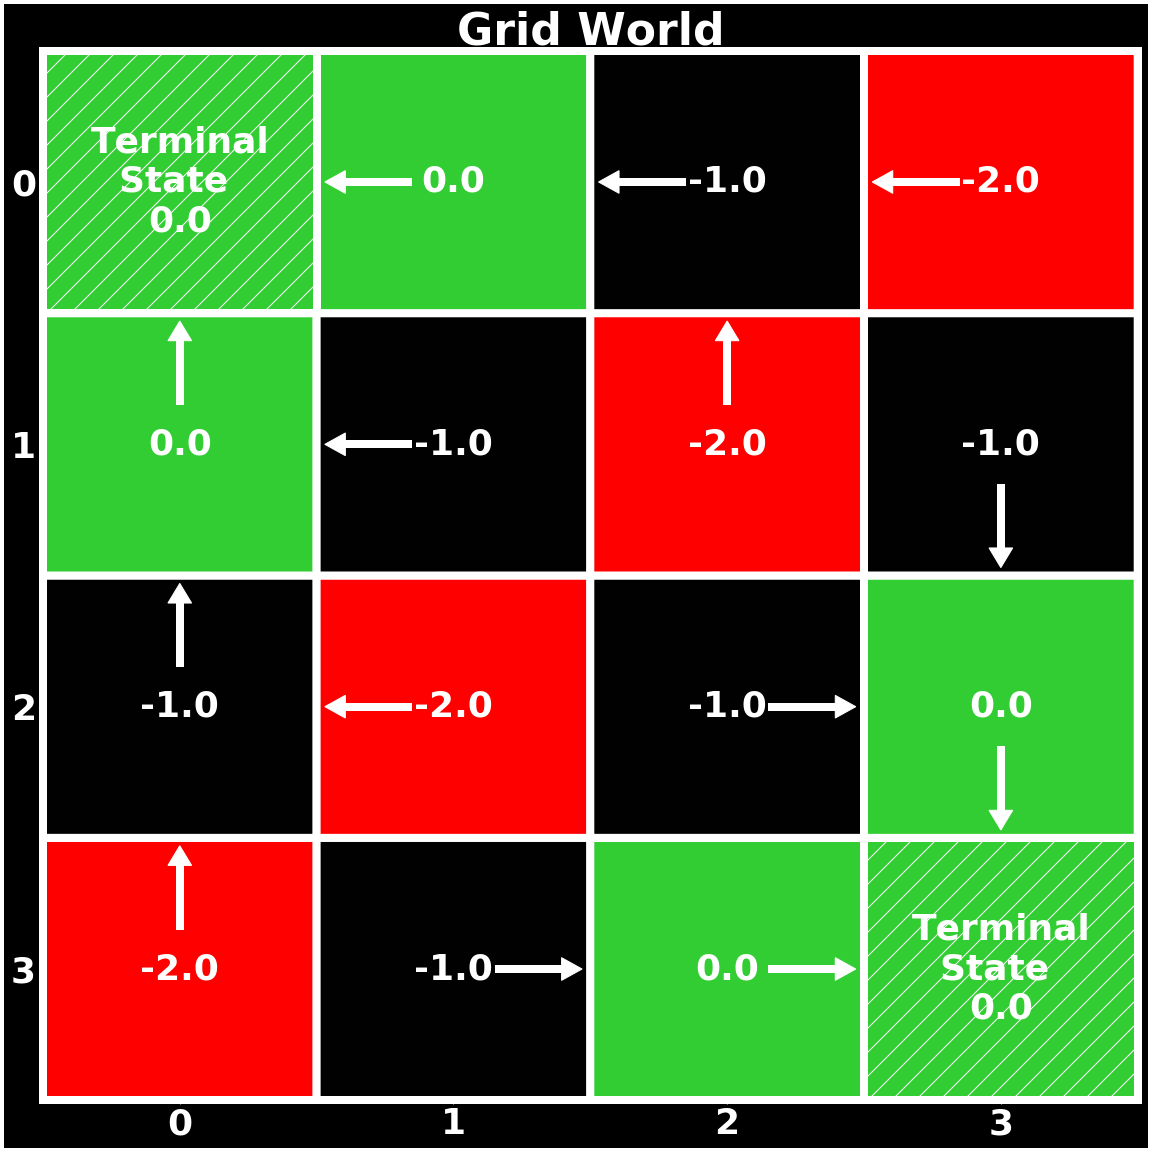
\includegraphics[width=.4\linewidth]{../paper_figs/value_iteration}}\hfill
    \subfloat[][$q$-value Iteration. Numbers represent the state-action values.\label{fig:q_value_iteration_simple}]{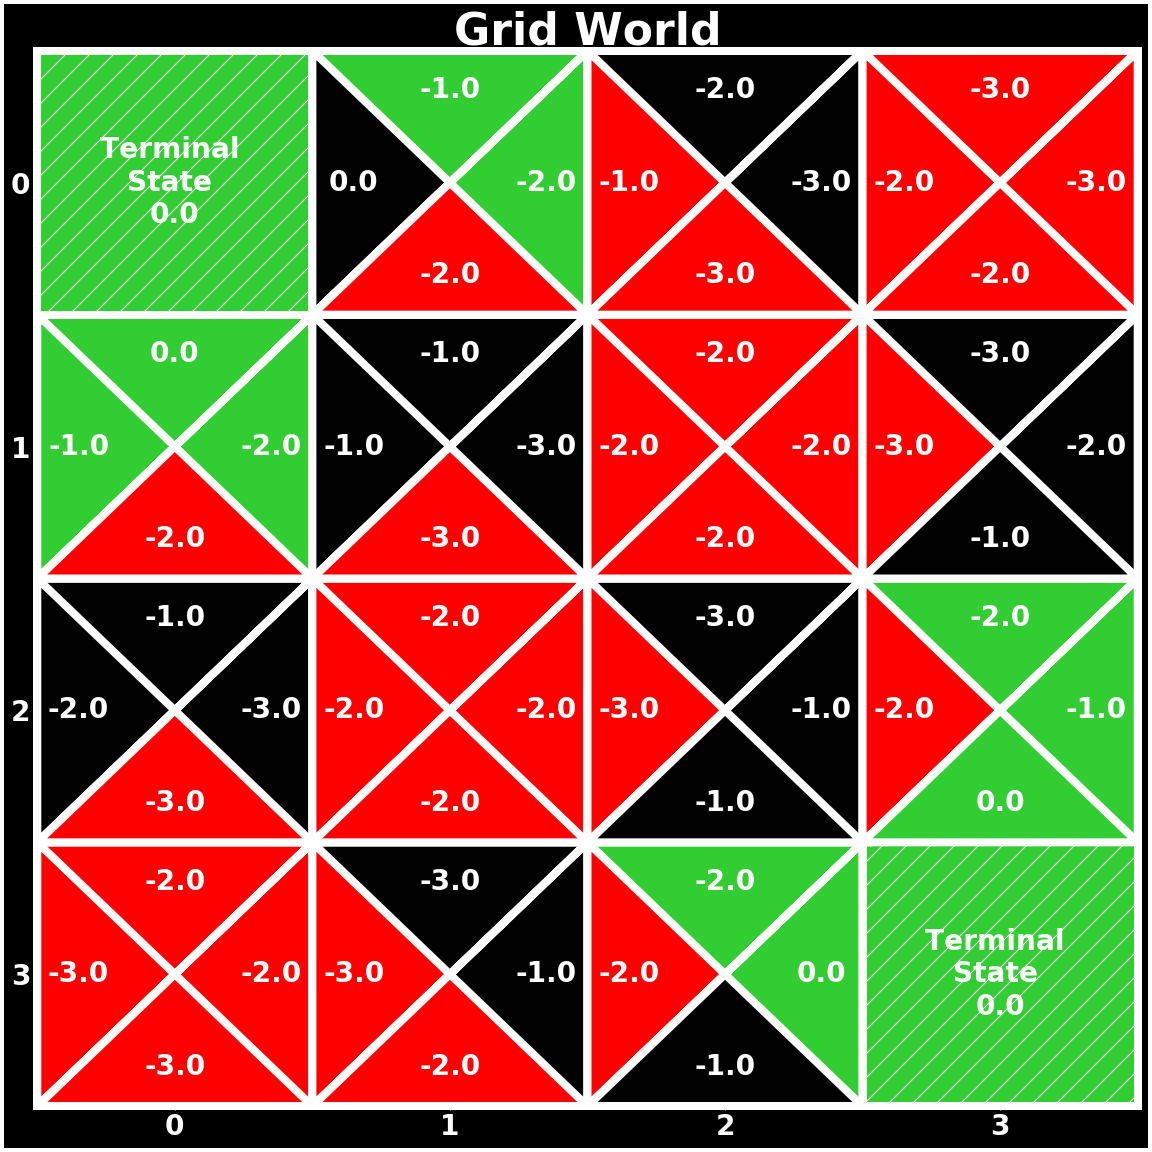
\includegraphics[width=.4\linewidth]{../paper_figs/q_value_iteration_simple}}
    \caption{Model based algorithms in grid-world.}
    \label{fig:model}
\end{figure}

Fig.~\ref{fig:model} illustrates the results of the model-based learning algorithms with value and policy iteration in Fig.~\ref{fig:value_iteration_simple} and $q$-value iteration in Fig.~\ref{fig:q_value_iteration_simple}. As was previously mentioned would be the case, each of these methods arrives at the same optimal policy. The evaluation criteria in this setting are the Bellman optimality conditions as well as the cumulative rewards of trials. Because this is a deterministic example we are able to satisfy the Bellman optimality conditions and we will always achieve the maximum possible reward in each trial as a result.

While the algorithms given in this section may appear as the be-all and end-all to RL given that we have shown they are optimal, in reality these methods have significant limitations. This is because as the state space grows very large dynamic programming methods become computationally intractable, creating the need for methods that approximate the Bellman optimality conditions. 

\section{Model Free Reinforcement Learning}\label{sec:model_free}
Model based dynamic programming methods face two significant limitations. As touched on previously, they become computationally intractable as the state space grows very large. Another limitation is that complete knowledge of the dynamics are required, yet transition probabilities and event outcomes are often unknown a priori in practice. To make up for these shortcomings, we turn our attention towards approximation methods that gradually improve estimates of the environment and the value functions. These methods are know as model free RL because they operate in an online fashion and require no knowledge at the outset of a problem.

The fundamental concept of model free RL is temporal-difference (TD) learning. TD methods are like dynamic programming methods in that they update value estimates using prior estimates before reaching a final outcome. The difference however, is that updates are made using sample feedback from the environment instead of the idealized model of the environment from the MDP. The TD error term for the state value function is given as follows
\begin{equation}\label{eq:td_v}
TD_v = R_{t+1} + \gamma V(S_{t+1}) - V(S_t),
\end{equation}
similarly the state-action value function is given by
\begin{equation}\label{eq:td_q}
TD_q = R_{t+1} + \gamma Q(S_{t+1}, A_{t+1}) - Q(S_t, A_t).
\end{equation}
These quantities may look familiar and indeed we can trace them back to a form of the Bellman equations from (\ref{eq:inter_v}) and (\ref{eq:inter_q}) which we restate for clarity here.
\begin{equation}\tag{\ref{eq:inter_v}}
v_\pi(s) = \mb{E}_\pi[R_{t+1} + \gamma v_\pi(S_{t+1})|S_t=s], 
\end{equation}
\begin{equation}\tag{\ref{eq:inter_q}}
q_\pi(s, a) = \mb{E}_\pi[R_{t+1} + \gamma q_\pi(S_{t+1}, A_{t+1})|S_t=s, A_t=a]
\end{equation}
It is now evident that the TD terms in equations (\ref{eq:td_v}) and (\ref{eq:td_q}) are sampling from the expected values of the targets from (\ref{eq:inter_v}) and (\ref{eq:inter_q}) and computing the error between the improved estimate of the value function with the current estimate of the value function. Intuitively the TD term can be interpreted as a gradient like term, which then lends naturally to the idea of algorithms using online stochastic gradient descent methods to improve value function estimates. It turns out in fact, that this is exactly how the most basic TD learning algorithms work. We have implemented the three core methods of TD(0), Sarsa, and $q$-learning. The methods differ by the policy that is being sampled from in the TD updates and whether a state value function or a state-action value function is being learned. 

TD(0) learns the state value function of a policy that is given. Meaning given policy $\pi$ the state value function $v_\pi$ is learned by sampling from $\pi$ and updating the state value function as follows:
\begin{equation}
V(S) = V(S) + \alpha [R' + \gamma V(S') - V(S)].
\end{equation}
Sarsa is an on-policy method, meaning that the policy being followed is the same as the policy being learned, that learns the optimal state-action value function. Typically, the $\epsilon$-greedy policy or the Boltzmann policy is followed. Each of these methods trades off exploration and exploitation. Given the greedy action $a^* = \arg \max_a Q(S, a)$ the $\epsilon$-greedy policy is given by
\begin{equation} \pi(a|s) =
\begin{cases}
\ 1 - \epsilon + \frac{\epsilon}{|A|} & a = a^* \\
\frac{\epsilon}{|A|} & a \neq a^*
\end{cases}
\end{equation}
where $\epsilon \in [0, 1]$ controls the greediness. The Boltzmann policy is given by
\begin{equation} \pi(a|s) =
\frac{e^{\tau Q(s, a)}}{\sum_a e^{\tau Q(s, a)}} 
\end{equation}
where $\tau$ is a temperature parameter $\in [0, \infty)$ that controls the greediness. It is common to use a decay rate on the parameters controlling the greediness to make the algorithm more greedy as the environment is further explored. We have implemented these policies in support of the algorithms. Given this information, the TD update in Sarsa is given as follows:
\begin{equation}
Q(S, A) = Q(S, A) + \alpha [R' + \gamma Q(S', A') - Q(S, A)].
\end{equation}
$q$-learning is very similar to Sarsa with the exception that it is an off-policy method, meaning that the policy being followed is different from the policy being learned, that learns the optimal state-action value function. Specifically $q$-learning follows the $\epsilon$-greedy policy or the Boltzmann policy but learns the greedy policy. The TD update is given as follows:
\begin{equation}
Q(S', A') = Q(S, A) + \alpha [R' + \gamma \max_a Q(S', a) - Q(S, A)].
\end{equation}

Finally, we note that to guarantee convergence of the temporal difference algorithms the Robbins and Monro conditions \cite{robbins1951stochastic} on the learning rate must hold
\begin{equation}
\sum_{t=0}^\infty \alpha_t(s, a) = \infty \hspace{5mm} \text{and} \hspace{5mm} \sum_{t=0}^\infty \alpha_t^2(s, a) < \infty, \ \forall \ s, a,
\end{equation}
and each state-action pair must be visited infinitely often during exploration (for more on convergence we refer the reader to \cite{tsitsiklis1994asynchronous} and \cite{sutton1998reinforcement}). While clearly this is infeasible, TD methods often reach a very good value function approximation and policy quickly. An example is the problem described in \ref{fig:model}, when testing the TD methods we find that the same optimal state value function and optimal policy is learned as the model based methods but in the state-action value function there is some error in the suboptimal state-action pairs. However, to an agent who wants to maximize their rewards, not estimating suboptimal values completely correct does not matter.

 \section{Risk-Sensitive Reinforcement Learning}\label{sec:risk}
The novel contribution of \cite{DBLP:journals/corr/ShenTSO13} was to extend the $q$-learning method by applying a transformation to the temporal difference term with a value function (note the conflation of the term value function, in this setting it means a type of function that maps utilities) obeying certain properties and coming from the class of functions that have been developed to model human behavior, while maintaining convergence guarantees. In particular the update in this algorithm is given by the following:
\begin{equation} 
Q(S, A) \gets Q(S, A) + \alpha[u(R + \gamma \max_a Q(S', a) - Q(S, A))].
\end{equation}
Through applying the value function to the temporal difference term, a nonlinear transformation is applied not only to the rewards, but also to the transition probabilities. This is significant given that this is precisely what humans have been observed to do when making decisions as we discussed in the introduction.

We explore and implement several functions that capture risk-sensitive decision making including a prospect theory value function \cite{tversky1992advances}, an entropic map value function, and a logarithm-based value function \cite{DBLP:journals/corr/RatliffM17}. We will focus on the prospect value function given by:
\begin{equation}u(y) = 
\begin{cases}
c_+ (x)^{\rho^+} & x > 0 \\
-c_- (-x)^{\rho^+} & x \leq 0 \\
\end{cases}
\end{equation}
where we are setting the reference point to be 0. The parameters $(c_+, c_-, \rho+, \rho_-)$ control the degree of risk-sensitivity and loss aversion. Typically human decision makers have $0 < \rho_+, \rho_- < 1$. In terms of the shape of the function these preferences correspond to concavity in gains and convexity in losses.

We now experiment with the value function in grid world using the configurations from Fig.~\ref{fig:prospect} to learn more about how risk-sensitivity influences the optimal value function and policy from a specific initial state. In this example we designate the state space to be indexes of the grid and actions to be the compass directions $\{N, E, S, W, NE, SE, SW, NW\}$. The transition function is configured such that an action results in the desired state with probability $.93$ and a random state with probability $.07$ except a terminal state is reached the agent remains there. All transitions incur a reward of $.1$ with the exception transitions to and from a terminal state incur a reward of $1$ for good terminal states and $-1$ for bad terminal states. The discount factor was set to $.95$. 
\begin{figure}[t]
    \centering
    \subfloat[][]{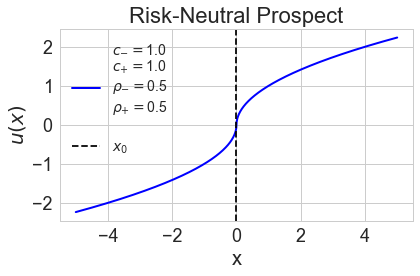
\includegraphics[width=.25\linewidth]{../paper_figs/prospect_neutral}\label{fig:risk1}}\hfill
    \subfloat[][]{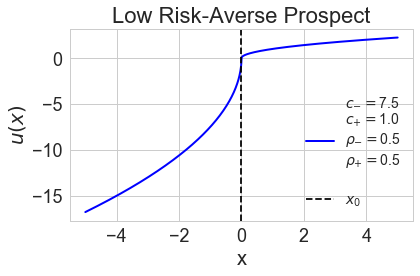
\includegraphics[width=.25\linewidth]{../paper_figs/prospect_low}\label{fig:risk2}}\hfill
    \subfloat[][]{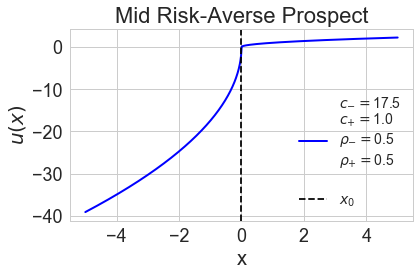
\includegraphics[width=.25\linewidth]{../paper_figs/prospect_mid}\label{fig:risk3}}\hfill
    \subfloat[][]{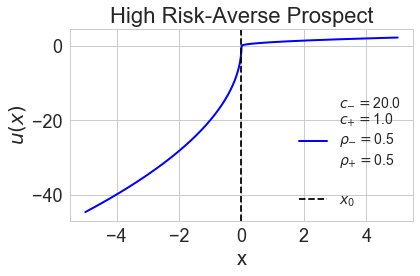
\includegraphics[width=.25\linewidth]{../paper_figs/prospect_high}\label{fig:risk4}}
    \caption{Prospect Theory value functions with varying risk-sensitivity parameters. In particular we fix ($c_+=1, \rho+=.5, \rho_-=.5$) and vary $c_- \in \{1, 7.5, 17.5, 20\}$ to produce the functions from left to right.}
    \label{fig:prospect}
\end{figure}
\vspace{-2mm}
\begin{figure}[H]
    \centering
    \subfloat[][Risk-Neutral.]{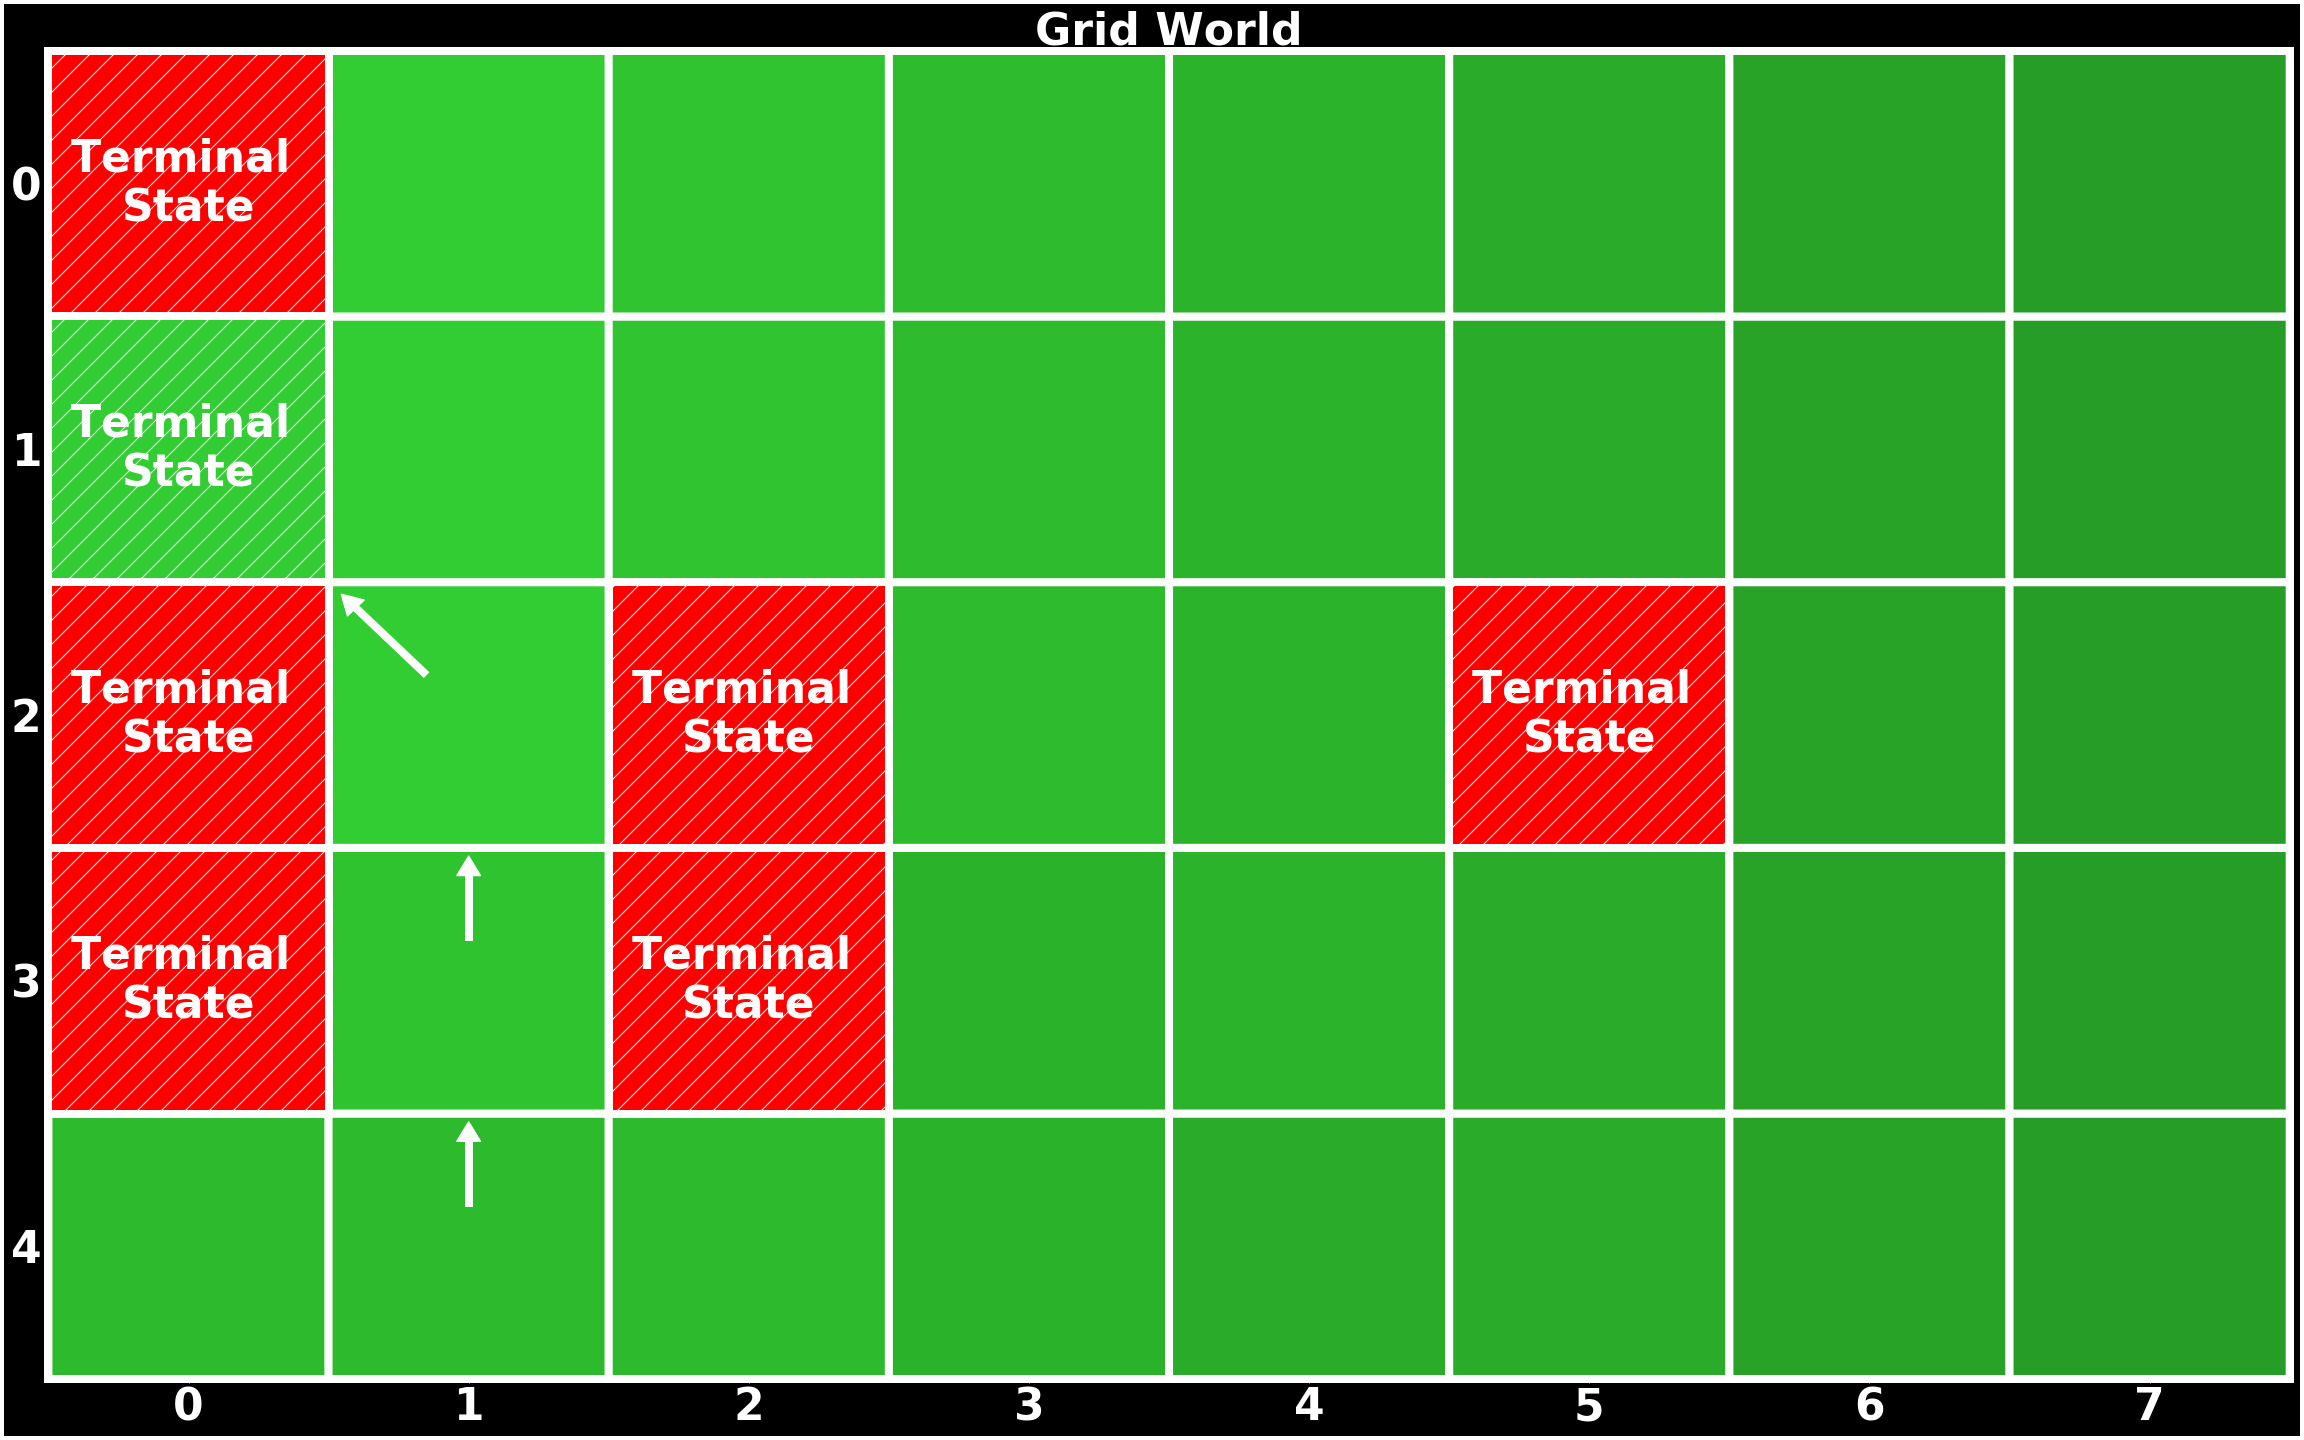
\includegraphics[width=.45\linewidth]{../paper_figs/policy_neutral}\label{fig:risk1_}}
    \subfloat[][Low Risk-Averse.]{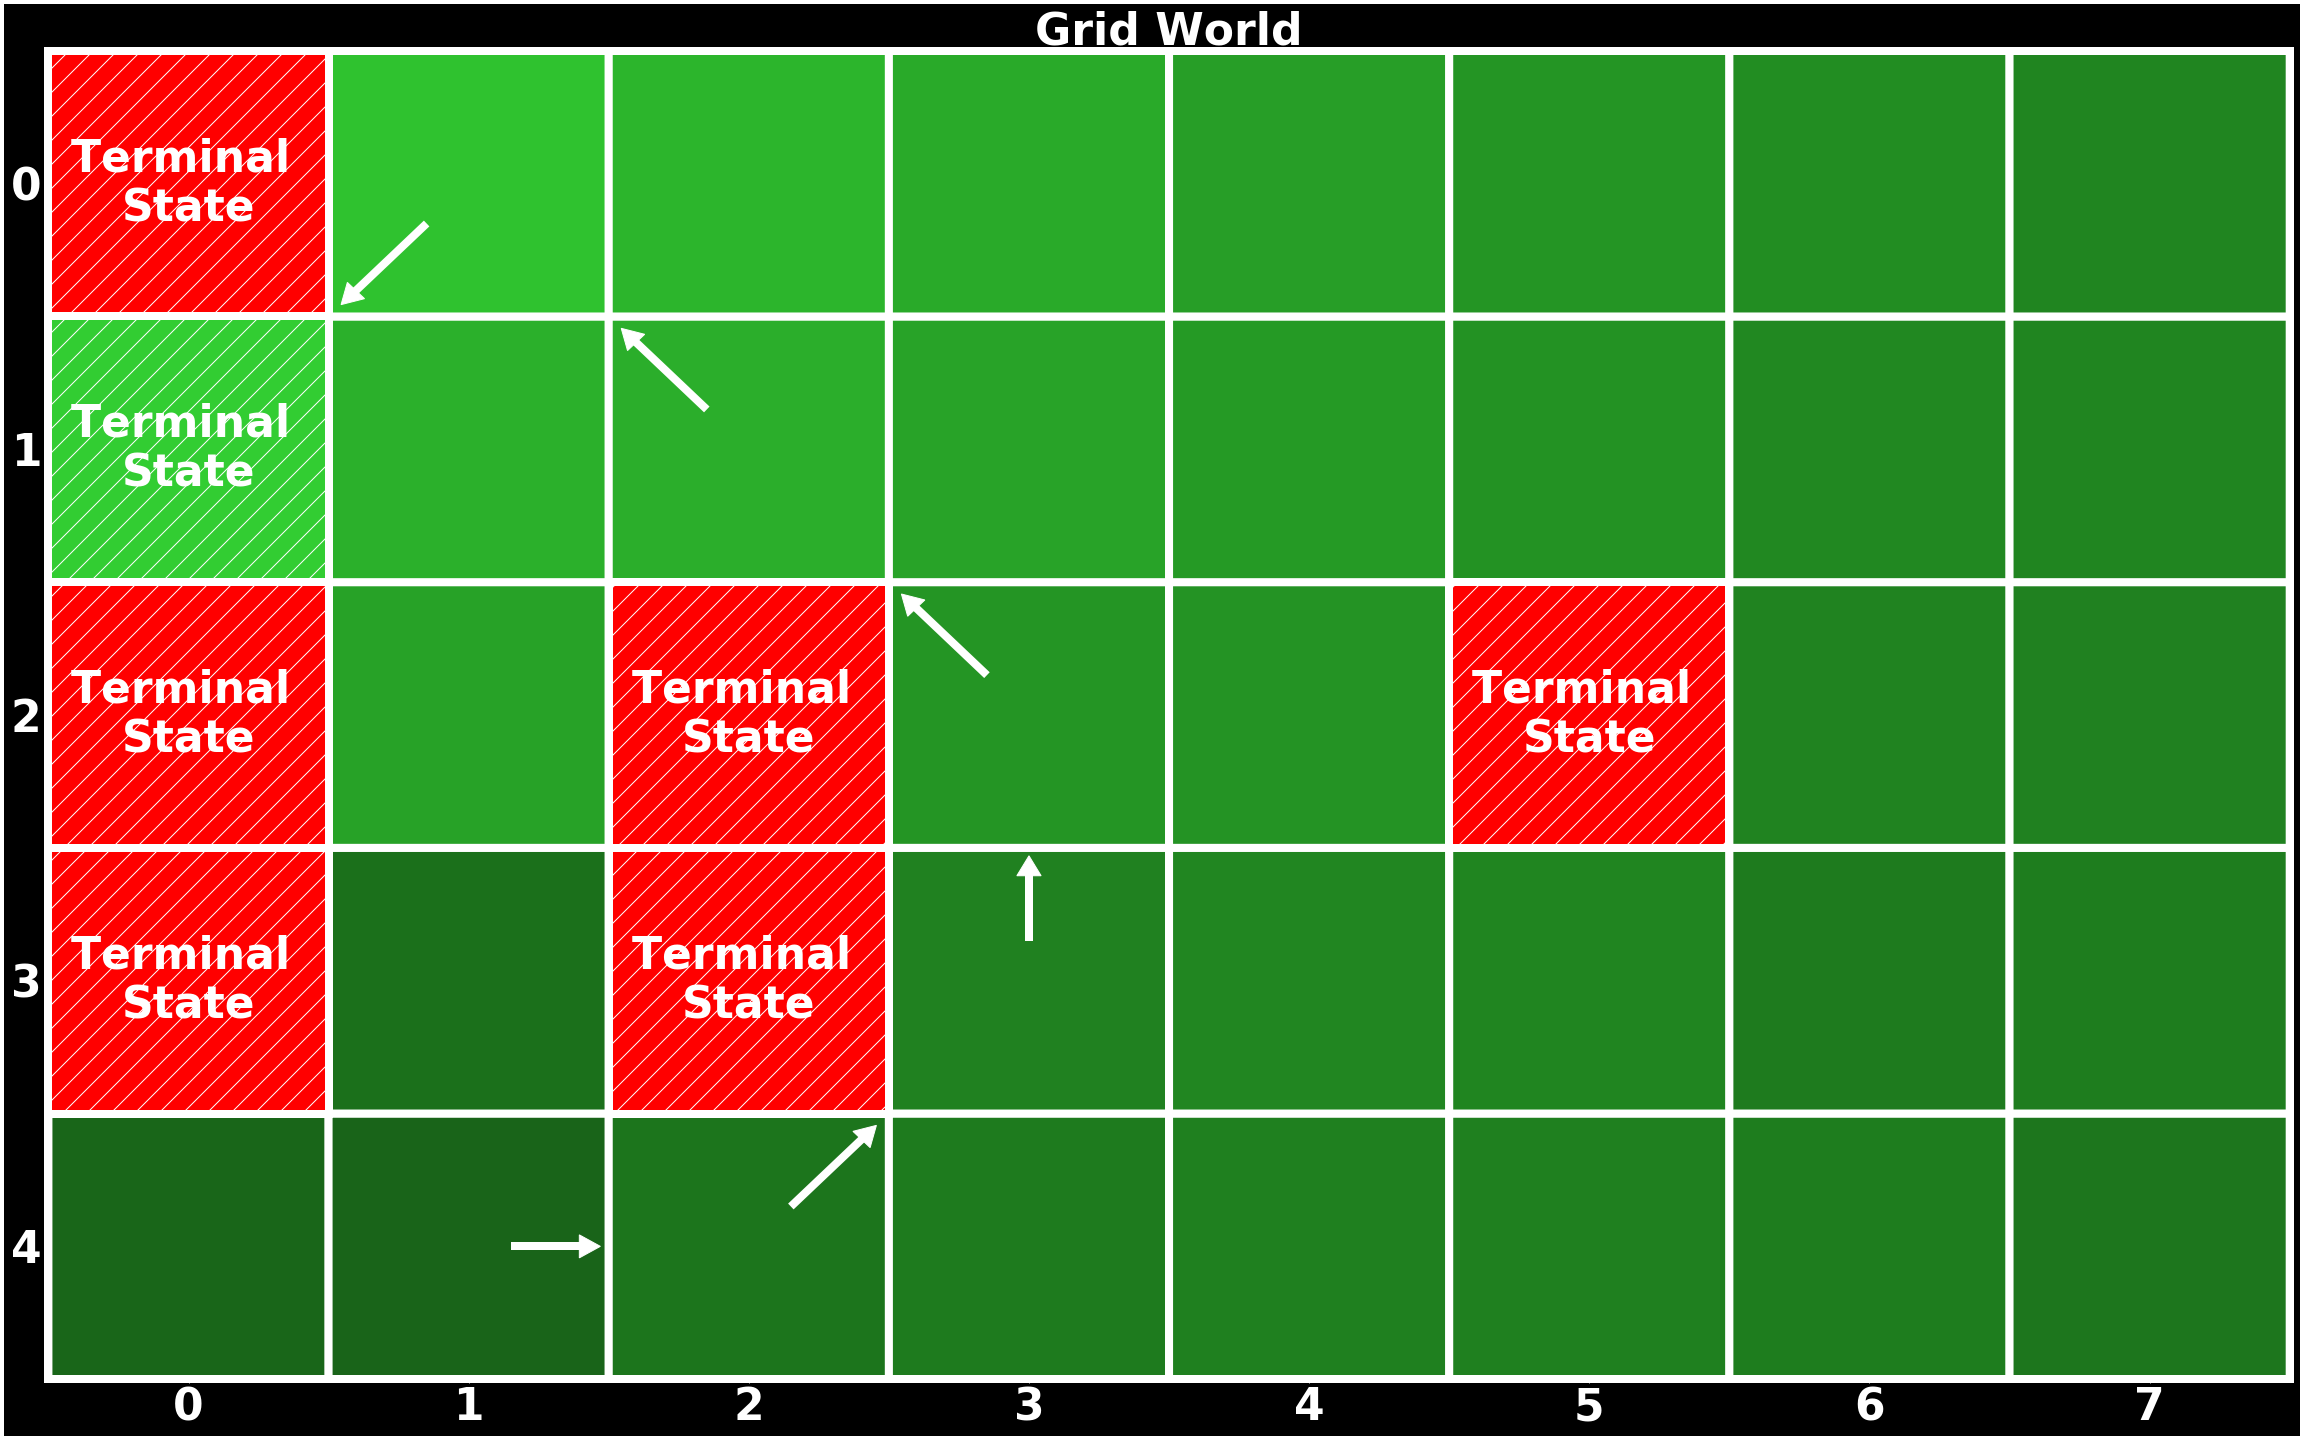
\includegraphics[width=.45\linewidth]{../paper_figs/policy_low}\label{fig:risk2_}}\vfill
    \subfloat[][Mid Risk-Averse.]{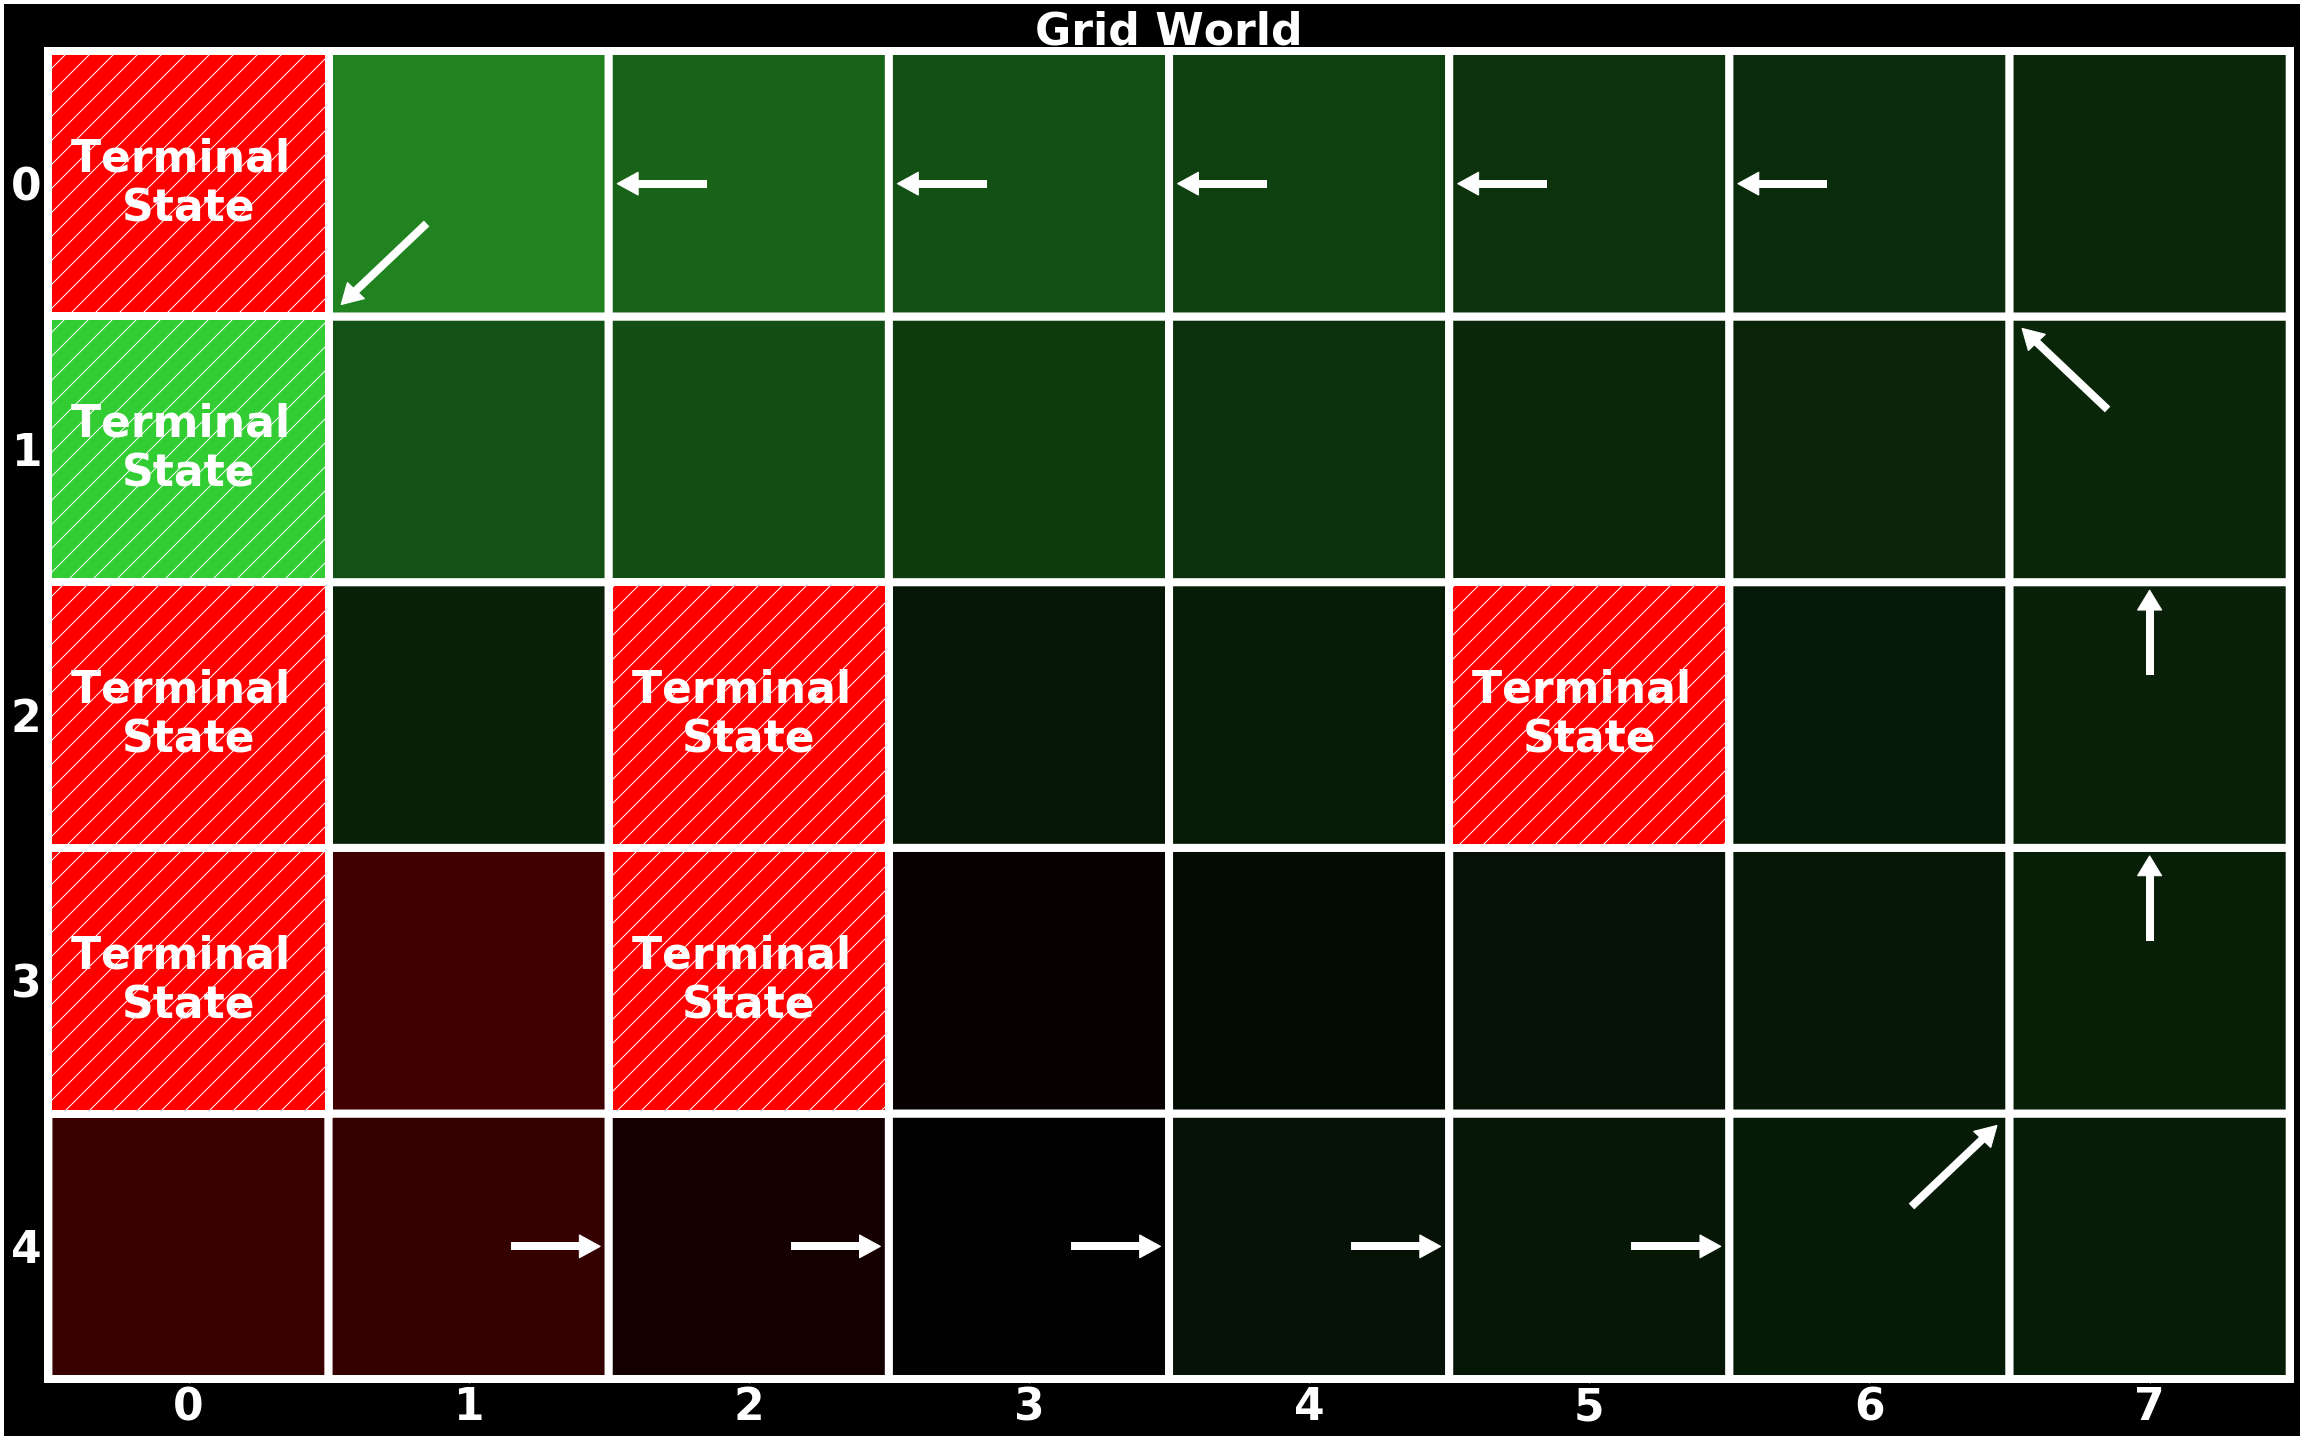
\includegraphics[width=.45\linewidth]{../paper_figs/policy_mid}\label{fig:risk3_}}
    \subfloat[][High Risk-Averse.]{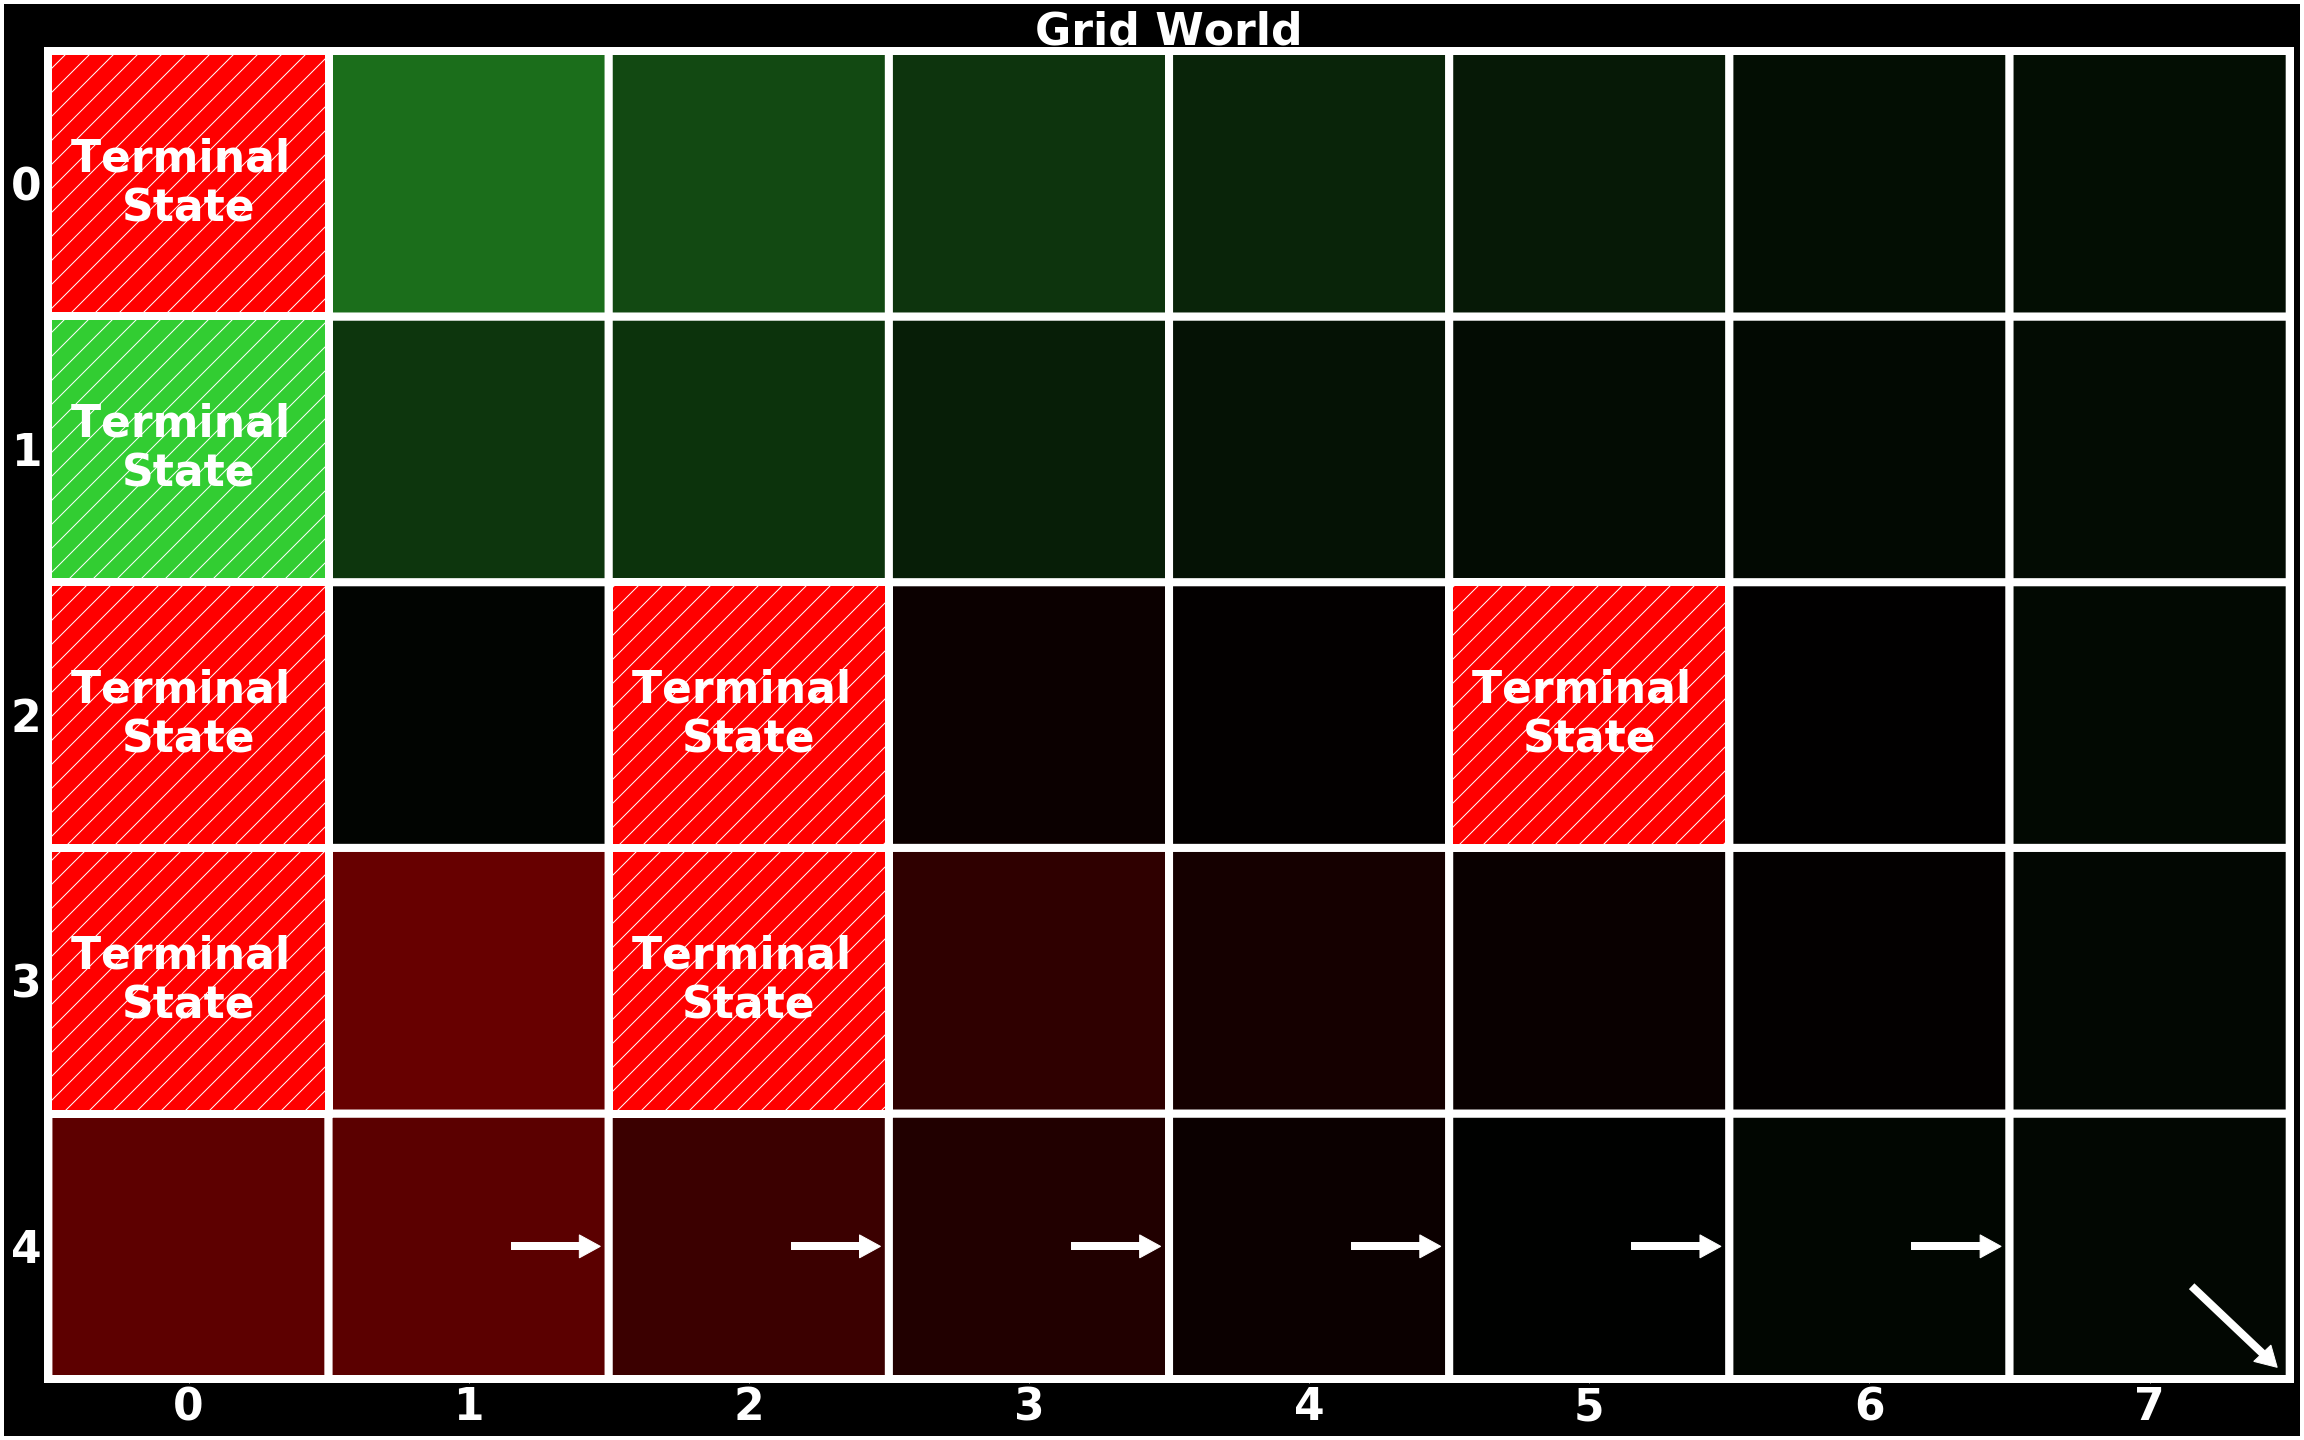
\includegraphics[width=.45\linewidth]{../paper_figs/policy_high}\label{fig:risk4_}}
    \caption{Risk-Sensitive $q$-learning results with varying risk-sensitivity parameters.}
    \label{fig:risk}
\end{figure}
\vspace{-2mm}
We see in Fig.~\ref{fig:risk} that a risk-neutral agent is not influenced by the small probability of going into a bad terminal state, but as the agent becomes risk averse they work to avoid the bad terminal states at growing levels by taking longer, safer paths to the good terminal state until they learn to stay far away from the bad terminal states and only collect a small reward. For the complete algorithm and additional details see Appendix Section~\ref{sec:risk_appendix}.

\section{New York Taxi Dataset}\label{sec:taxi}
We formulate the decision process of a taxi driver as a MDP in order to learn the optimal policy to maximize earning rates as well as compare to empirical polices from data to see how well the drivers do at present.

The New York Taxi Dataset covers taxi operations from $2010$--$2013$. The key information that is contained is the hack license (driver ID), pickup date-time, dropoff date-time, trip time in seconds, trip distance in miles, GPS coordinates at starting and ending locations, total fare including tip, and the total cost of tolls. The data required a significant amount of preprocessing to clean the data and obtain the needed quantities for the MDP formulation. In fact, it was estimated by \cite{donovan2014new} that nearly $10\%$ of trips contained erroneous information. We gave particular attention to cleaning incorrect trip times, as well as infeasible trip locations, distances, and earning rates.


The complete formulation of the finite MDP for a taxi driver we derived is detailed in Appendix Section \ref{mdp}. The salient features of the formulation are:
\begin{itemize}
\item Each state is a tuple containing the node the driver is in--we discretized location into a grid using district boundaries for New York City--an indicator of whether the taxi currently is full (just picked up passengers) or empty (just dropped off passengers), and the cumulative reward interval the driver is in--we discretized the reward intervals assuming that how a driver behaves may be a function of the earnings at a point in the workday.
\item Actions are moving between nodes in the location grid we created.
\item The reward functions use values derived from the data, such as earning rate, the expected time searching for a passenger, and the fare between grid nodes. The transition probabilities use empirical transition probabilities as well as expected earning rates. 
\item The policy is given by the actions taken when looking to pick up new passengers, i.e. empty to full transitions.
\end{itemize} 

There are also a couple of important things we do to create the MDP which we make note of. Drivers work abnormal hours, i.e. the typical driver begins work in the evening and works until the early morning hours. In light of this we shift all transaction times back by 12 hours so that we can observe the full workday within a single date. We estimate the time spent searching for a new trip as the time from dropoff to pickup, but if this time exceeds 20 we assume the driver was taking a break.

We select 7 drivers and analyze then over a three month period in 2010. For each driver we solve the MDP using one of our model based RL algorithms and  compare the empirical policy to the optimal policy for several discount factors.
\vspace{-2mm}
\begin{table}[H]
\centering
\caption{Percentage of decision states (empty to full and not in a terminal state)} that the empirical policy matches the optimal policy learned.
\label{my-label}
\begin{tabular}{|c|c|c|c|c|c|c|c|c|}
\hline
DriverID & 1 & 2 & 3 & 4 & 5 & 6 & 7 \\
\hline
$\gamma = .9$ & 59.3 & 51.7 & 32.2 & 34.1 & 33.3 & 28.6 & 44.7 \\
$\gamma = .95$ & 60.0 & 44.4 & 17.2 & 21.8 & 26.0 & 16.4 & 36.7 \\
$\gamma = 1$ & 75.0 & 75.6 & 77.8 & 84.7 & 63.3 & 86.4 & 64.7 \\
\hline
\end{tabular}
\end{table}
\vspace{-2mm}
The results show that drivers do not act optimally. Interestingly they are closest to the policy learned with a discount factor of 1. In this case the policy learned was nearly always to stay in the same grid location to look for rides. As the discount factor decreased we saw increased occurrences in the learned policy of going to the grid locations that contained one of the airports. We believe this is because there are longer trips and higher earning rates but this comes at the cost of lost time in traveling there with no ride.
\section{Conclusions and Future Work}
In this project we thoroughly analyzed finite MDPs and RL theoretically and computationally by developing a significant code base of algorithms and infrastructure for experimentation. We also explored an interesting RL paradigm of risk-sensitivity and concluded with formulating the decision process of a taxi driver as an MDP. In future work we would like to apply the risk-sensitive RL to the taxi problem and tune parameters to try and find a policy that matches the empirical policy closely, which would tell us the risk-preferences a driver was acting on.

\bibliographystyle{unsrtnat}
\bibliography{bibtex}


\newpage
{\center\Large\bfseries APPENDIX\par}
\renewcommand\thesection{\Alph{section}}
\setcounter{section}{0}

\section{Implementation Details}\label{imp_appendix}
All functionality in this project was implemented on our own without the use of machine learning packages. The framework we have developed allows for testing and comparison of many RL algorithms in only a few simple lines of code thanks to the object oriented structure, much like scikit-learn. For evaluation purposes we have created a grid-world environment and made our framework compatible with OpenAI Gym. 

The salient features is that we divide up RL approaches into model based, model free, and risk-sensitive and develop classes for each. Since the approaches share many features and we would like to be able to test optimality and visualize results all the same, it is natural that these are derived from base classes. When instantiating one of the objects there are parameters for that can be chosen such as the learning rate, policy type, and decay parameters.

The grid-world environment we created takes in parameters allowing for specification of the states, actions, transition probabilities, and rewards in a very simple way. Moreover it allows for extremely clear visualizations of state value functions, state-action value functions, and policies that are appealing to they eye. 

Below we demonstrate how easy it is to use and test the RL algorithms in grid-world with our code. This is how we created the examples in Section~\ref{sec:model_based} of model based algorithms in grid-world.
\begin{lstlisting}
import RL

# Problem specifications.
grid_rows = 4
grid_cols = 4
num_actions = 4
living_rewards = -1
terminal_states = [0, 15]
terminal_rewards = {0:0, 15:0}

# Creating the MDP.
mdp = RL.GridWorldMDP(grid_rows, grid_cols, num_actions, terminal_states, 
                      terminal_rewards, prob_noise=.0, 
                      living_rewards=living_rewards, reward_into=False)


# Creating the model based RL object.
model_rl = RL.ModelBasedRL()

# Run, visualize, and test for optimality of policy iteration.
model_rl.policy_iteration(mdp)
display = RL.GridDisplay(model_rl, mdp)
display.show_values(fig_name='policy_iteration.png', save_fig=True)
v_error = model_rl.test_optimal_v(mdp)

# Run, visualize, and test for optimality of value iteration.
model_rl.value_iteration(mdp)
display = RL.GridDisplay(model_rl, mdp)
display.show_values(fig_name='value_iteration.png', save_fig=True)
v_error = model_rl.test_optimal_v(mdp)

# Run, visualize, and test for optimality of q-value iteration.
model_rl.q_value_iteration(mdp)
display = RL.GridDisplay(model_rl, mdp)
display.show_q_values(fig_name='q_value_iteration.png', save_fig=True)
q_error = model_rl.test_optimal_q(mdp)
v_error = model_rl.test_optimal_v(mdp)
\end{lstlisting}
Like in grid world we can apply any of the methods described in this paper in OpenAI Gym. An example on a task of picking up a passenger and moving them to a desired location in a grid is shown below using both model free methods, and model based methods where we use an estimated MDP that is learned from interacting with the environment.
\begin{lstlisting}
import gym
import RL

# Gym environment to learn.
env = gym.make('Taxi-v2')

# We simulate the env so we can estimate an MDP to apply model based RL to.
mdp = RL.SimulatedMDP(env)


# Apply value iteration.
model_rl.value_iteration(mdp)

# Simulate using the policy that was learned and the last episode is displayed.
model_rl.simulate_policy(env)

# Plotting the returns at each episode.
model_rl.scatter_epsiode_returns()


# Creating parameters needed for ModelFreeRL class.
n = env.observation_space.n
states = range(n)
m = env.action_space.n
actions = range(m)

# Creating model free RL object.
model_free_rl = RL.ModelFreeRL(n=n, m=m, states=states, actions=actions)

# Running the q-learning algorithm.
model_free_rl.q_learning(env)

# Plotting the returns, epsilon choices, and alpha parameters at each episode.
model_free_rl.plot_epsiode_returns()
model_free_rl.plot_epsilon_parameters()
model_free_rl.plot_alpha_parameters(s=0, a=0)

# Simulate using the policy that was learned and the last episode is displayed.
model_free_rl.simulate_policy(env)
\end{lstlisting}

\section{Risk-Sensitive Decision Making Example}\label{example}
A prevalent example to demonstrate how risk factors into human-decision making including warping of the probability of events as well as losses being weighed more significantly than gains is as follows. When asked to choose between being given \$90 or having a 10\% chance of winning \$100 and a 90\% chance of winning \$0 most people will choose to take the guaranteed \$90. When this question is framed as a loss however, i.e. to choose between losing \$90 or having a 10\% chance of losing \$0 and a 90\% chance of losing \$100, most will choose to risk an increased loss for a chance at no loss. A rational, risk-neutral decision maker would be indifferent to the options in both framings of the question since the expected value of each option is the same.

\section{Bellman Optimality Conditions Derivation}\label{bellman}
The bellman optimality conditions represent that the value of a state under an optimal policy must be equal to the expected return for the best action from the state. The derivations follow from the Bellman equations.
\begin{equation*}
\begin{split}
v_*(s) &= \underset{a \in A}{\text{max}} \ q_{\pi_*}(s,a) \\
&= \underset{a}{\text{max}} \ \mathbb{E}_{\pi^*}[\sum_{k=0}^\infty \gamma^k R_{t + k+ 1}|S_t = s, A_t =a] \\
&= \underset{a}{\text{max}} \ \mathbb{E}_{\pi^*}[R_{t+1} + \gamma \sum_{k=0}^\infty \gamma^k R_{t + k+ 2}|S_t = s, A_t =a] \\
&= \underset{a}{\text{max}} \ \mathbb{E}[R_{t+1} + \gamma v_*(S_{t+1})|S_t = s, A_t =a] \\
&= \underset{a}{\text{max}} \ \sum_{s', r'}p(s', r'|s,a)[r' + \gamma v_*(s')], \\
\end{split}
\end{equation*}
The bellman optimality equation for $q_*$ is then 
\begin{equation*}
\begin{split}
q_*(s,a) &= \mathbb{E}[R_{t+1} + \gamma \underset{a'}{\text{max}} \ q_*(S_{t+1}, a')|S_t =s, A_t=a] \\
&= \sum_{s', r'}p(s', r'|s,a)[r' + \gamma \underset{a'}{\text{max}} \ q_*(s',a')].
\end{split}
\end{equation*}

\section{Model Based RL Algorithms}\label{sec:model_appendix}
\begin{algorithm}[H]
\caption{Policy Iteration}
\begin{spacing}{0.8}
\begin{algorithmic}[1]
\Procedure{PolicyIteration}{}
\State \textbf{Initialize:} $v(s) = 0, \ \forall \ s \in \mc{S}, \pi(s) \in \mc{A} \ \forall \ s \in \mc{S}$
\State 1. Policy Evaluation
\While{$\text{True}$}
\State $\delta \gets 0$ 
\For{$s \in \mc{S}$}
\State $v_{temp} \gets v(s)$
\State $v(s) \gets \sum_{s', r'}p(s', r'|s,\pi(s))[r(s,a,s') + \gamma v(s')]$
\State $\delta \gets \text{max}(\delta, |v_{temp} - v(s)|)$
\EndFor
\If{$\delta < \epsilon$}
\State \text{break}
\EndIf
\EndWhile
\newline
\State 2. Policy Improvement
\State stable $\gets$ True
\For{$s \in \mc{S}$}
\State $\text{old-action} \gets \pi(s)$
\State $\pi(s) \gets \arg \max_a \sum_{s',r'} p(s', r'|s,a)[r(s,a,s') + \gamma v(s')]$
\If{old-action $\neq \pi(s)$}
\State stable $\gets$ False
\Else
\State Begin again at 1.
\EndIf
\EndFor
\If{stable}
\State return $v, \pi$ and end
\EndIf
\EndProcedure
\end{algorithmic}
\end{spacing}
\end{algorithm}


\begin{algorithm}[H]
\caption{Value Iteration}
\begin{spacing}{0.8}
\begin{algorithmic}[1]
\Procedure{ValueIteration}{}
\State \textbf{Initialize:} $v(s) = 0, \ \forall \ s \in \mc{S}$
\While{$\text{True}$}
\State $\delta \gets 0$ 
\For{$s \in \mc{S}$}
\State $v_{temp} \gets v(s)$
\State $v(s) \gets \underset{a}{\text{max}} \sum_{s', r'}p(s',r'|s,a)[r(s,a,s') + \gamma v(s')]$
\State $\delta \gets \text{max}(\delta, |v_{temp} - v(s)|)$
\EndFor
\If{$\delta < \epsilon$}
\State \text{break}
\EndIf
\EndWhile
\State $\pi \gets \underset{a}{\text{argmax}} \ \sum_{s',r'} p(s',r'|s,a)[r(s,a,s') + \gamma v(s')], \ \forall \ s \in \mc{S}$
\EndProcedure
\end{algorithmic}
\end{spacing}
\end{algorithm}

\begin{algorithm}[H]
\caption{Q Value Iteration}\label{euclid}
\begin{spacing}{0.8}
\begin{algorithmic}[1]
\Procedure{QValueIteration}{}
\State \textbf{Initialize:} $q(s, a) = 0, \ \forall \ s \in \mc{S}, a \in \mc{A}$
\While{$\text{True}$}
\State $\delta \gets 0$ 
\For{$s \in \mc{S}, a \in \mc{A}$}
\State $q_{temp} \gets q(s, a)$
\State $q(s, a) \gets \sum_{s', r'}p(s',r'|s,a)[r(s,a,s') + \gamma \max_a q(s', a')]$
\State $\delta \gets \text{max}(\delta, |q_{temp} - q(s, a)|)$
\EndFor
\If{$\delta < \epsilon$}
\State \text{break}
\EndIf
\EndWhile
\State $\pi \gets \underset{a}{\text{argmax}} \ q(s), \ \forall \ s \in \mc{S}$
\EndProcedure
\end{algorithmic}
\end{spacing}
\end{algorithm}

\section{Model Free RL Algorithms}\label{sec:model_free_appendix}
\begin{algorithm}[H]
\caption{TD(0)}
\begin{spacing}{0.8}
\begin{algorithmic}[1]
\Procedure{TD(0)}{}
\State \textbf{Initialize:} $V(s) = 0, \ \forall \ s \in \mc{S}$
\For{each episode}
\State Initialize S
\For{step in episode}
\State $A \gets \text{action given by $\pi$ for $S$}$
\State Take action $A$, observe $R, S'$
\State $V(S) \gets V(S) + \alpha[R + \gamma V(S') - V(S)]$
\State $S \gets S'$
\EndFor
\State Until end of the horizon or episode.
\EndFor
\EndProcedure
\end{algorithmic}
\end{spacing}
\end{algorithm}

\begin{algorithm}[H]
\caption{Sarsa}
\begin{spacing}{0.8}
\begin{algorithmic}[1]
\Procedure{Sarsa}{}
\State \textbf{Initialize:} $Q(s, a) = 0 \ \forall \ s \in \mc{S}, a \in \mc{A}$
\For{each episode}
\State Initialize S
\State Choose A from S using policy derived from Q (e.g., $e$-greedy or Boltzmann)
\For{step in episode}
\State Take action $A$, observe $R, S'$
\State Choose A$'$ from S$'$ using policy derived from Q (e.g., $e$-greedy or Boltzmann)
\State $Q(S, A) \gets Q(S, A) + \alpha[R + \gamma Q(S', A') - Q(S, A)]$
\State $S \gets S'$
\EndFor
\State Until end of the horizon or episode.
\EndFor
\EndProcedure
\end{algorithmic}
\end{spacing}
\end{algorithm}

\begin{algorithm}[H]
\caption{Q-Learning}
\begin{spacing}{0.8}
\begin{algorithmic}[1]
\Procedure{Q-Learning}{}
\State \textbf{Initialize:} $Q(s, a) = 0 \ \forall \ s \in \mc{S}, a \in \mc{A}$
\For{each episode}
\State Initialize S
\For{step in episode}
\State Choose A from S using policy derived from Q (e.g., $e$-greedy or Boltzmann)
\State Take action $A$, observe $R, S'$
\State $Q(S, A) \gets Q(S, A) + \alpha[R + \gamma \max_a Q(S', a) - Q(S, A)]$
\State $S \gets S'$
\EndFor
\State Until end of the horizon or episode.
\EndFor
\EndProcedure
\end{algorithmic}
\end{spacing}
\end{algorithm}

\section{Risk-Sensitive Reinforcement Learning}\label{sec:risk_appendix}
\begin{algorithm}[H]
\caption{Risk-Sensitive Q-Learning}
\begin{spacing}{0.8}
\begin{algorithmic}[1]
\Procedure{Risk-SensitiveQ-Learning}{}
\State \textbf{Initialize:} $Q(s, a) = 0 \ \forall \ s \in \mc{S}, a \in \mc{A}$
\For{each episode}
\State Initialize S
\For{step in episode}
\State Choose A from S using policy derived from Q (e.g., $e$-greedy or Boltzmann)
\State Take action $A$, observe $R, S'$
\State $Q(S, A) \gets Q(S, A) + \alpha[u(R + \gamma \max_a Q(S', a) - Q(S, A))]$
\State $S \gets S'$
\EndFor
\State Until end of the horizon or episode.
\EndFor
\EndProcedure
\end{algorithmic}
\end{spacing}
\end{algorithm}


\section{Taxi MDP Model Description}\label{mdp}
\subsection{State Space}
The state space is
\[\mc{X}=\{\mc{N}\cup\{x_f\}\times\mc{S}\times \mc{R}\}\backslash \mc{X}_{na}\]
where
\begin{itemize}
\item $x_f$ is the terminal state representing the taxi being done for the period,

\item $\mc{N}$ be the index set for the zones or nodes in the city with $N$ nodes. We use boundaries from the city of New York that divide up the city into approximately 200 neighborhoods. Because the overwhelming percentage of rides begin in small set of states we aggregate this to 10 nodes,

\item $\mc{S}=\{${\e, \f}$\}$ is an indicator of if the taxi is \e=empty or \f=full, and

\item $\mc{R}$ is the discretized cumulative fare value space which has the
structure \[\mc{R}=\{\mc{R}_1\}\cup\cdots\cup\{\mc{R}_m\}\cup\{\mc{R}_f\}\]
where $\mc{R}_i=[a_i,b_i]$ with $a_1< b_1\leq a_2<b_2 \cdots \leq a_m<
b_m=\bar{r}$ and $\mc{R}_f=[\bar{r}, \infty)$ where $\bar{r}$ is some reference point for period earnings (e.g., if the period of investigation is a day, then this is the daily earnings reference point which could be the median or mean). The purpose of this is to impose some structure on the problem owing to the thought that how a driver acts may be dependent on their cumulative earnings in the day. We use intervals of $\$20$ apart for our experiments.

\item $\mc{X}_{na}$ are the states not allowed and is defined by
\[\mc{X}_{na}=\{(x_f,\f,r), r\in \mc{R}\}\cup\{(x_f,\e,r), r\notin\mc{R}_f\}\]
\end{itemize}
   
A state $(i,s,r)\in \mc{N}\times\mc{S}\times \mc{R}$ indicates the taxi
is in node $i$ (or terminal state $x_f$ if $i=x_f$), has a empty/full state of $s$ and has current cumulative
fare value $r$. The terminal state is reached when the fare value portion of the
state is greater than or equal to $\bar{r}$. 

The dimension of the state space is thus, 
\[(\dim(\mc{N})+\dim(\{x_f\}))\times\dim(\mc{S})\times\dim(\mc{R})-|\mc{X}_{na}|.\]


\subsection{Action Space}
Let $\mc{U}=\mc{U}_a\cup\{\emptyset\}$ where
$\mc{U}_a=\{u_{i\mapsto j}, (i,j)\in \mc{N}\times \mc{N}\}$ be the action space where $u_{i\mapsto j}$ indicates the choice of going from node $i$ to node $j$ and where $\emptyset$ is the null action. The admissible actions are state dependent. In particular, if the state is $x=(i,\e,r)$ for any $i\in
\mc{N}$ and any cumulative fare value $r\in\mc{R}$, then $\mc{U}(i,\e,r)=\{u_{i\mapsto j}, (i,j)\in \mc{N}\times \mc{N}\}$ and, on the other hand, if $x=(i,\f,r)$ for any $i\in \mc{N}$ and any cumulative fare value $r\in\mc{R}$, then
$\mc{U}(i,\f,r)=\{\emptyset\}$ indicating that the taxi is currently full and is taking a ride from node $i$ to node $k$ with probability $\Pdest(i,k)$ (i.e.~the probability that a fare picked up in node $i$ will want to go to node $k$).

\subsection{Transition Kernel}
Let $\mc{P}: \mc{X}\times \mc{U}\times\mc{X}\rar [0,1]$ be the transition kernel such that $\mc{P}(x_{t},u_t, x_{t+1})$ is the probability that state $x_t$ will transition to state $x_{t+1}$ given action $u_t$. Let's consider the different cases. 
\begin{itemize}
\item First let's look at the $\e$ to $\e$ transitions for all other state action pairs:
\[\mc{P}( (i,\e,r),u,(j,\e,r'))=\left\{\begin{array}{ll} 1, & \ \text{if}\ r,r'\in \mc{R}_f\ \text{\&}\ \{i\in \mc{N},j=x_f\}\vee\{i=x_f,j=x_f\}\\
0, & \ \text{otherwise}\end{array}\right.\]

\item Now let's look at the $\f$ to $\f$ transitions for all other state action pairs:

\[\mc{P}( (i,\f,r),u,(j,\f,r'))=0\]
\item Next we will look at the $\f$ to $\e$ transitions for all other state action pairs:
\[\mc{P}((i,\f,r),u,(j,\e,r'))=\left\{\begin{array}{ll}
\Pdest(i,j)P(E[F(i,j)]+r\geq a_l)\ & \ \text{if}\ r'\in \mc{R}_l, r'\geq r\ \text{\&}\ i,j\in \mc{N}\\ 0, & \ \text{otherwise} \end{array}\right.\]
where $a_l$ is the lower bound on the interval
$\mc{R}_l=[a_l,b_l)$
\item Finally we look at the $\e$ to $\f$ transitions (these are all ones where the choices of action dictates the transition probability)

\[\mc{P}( (i,\e,r),u,(j,\f,r'))=\left\{\begin{array}{ll} 1, & \ \text{if}\ u=u_{i\mapsto j}\ \text{\&}\ r=r', r\notin \mc{R}_f\\
0, & \ \text{otherwise}\end{array}\right.\]
\end{itemize}

\subsection{Reward Function}
The reward function is a map $R:\mc{X}\times \mc{U}\times \mc{X}\times \rar \mb{R}$ with $R(x_{t},u_t,x_{t+1})$ a random variable such that
\begin{itemize}
\item The reward for $\f$ to $\e$ is 

\[R( (i,\f,r), u, (j,\e,r'))=\left\{\begin{array}{ll}F(i,j), & \ \text{if}\ i,j\in \mc{N}, u=\emptyset, r'\geq r, r' \notin \mc{R}_f\\ 
1000, & \ \text{if}\ i,j\in \mc{N}, u=\emptyset, r'\geq r, r' \in \mc{R}_f\\ 
0, & \ \text{otherwise}\end{array}\right.\]
where $F(i,j)$ is a random variable representing the fare from $i$ to $j$. The very large reward in designed to encourage the learning algorithm to determine that the ultimate goal is to reach a cumulative earnings threshold. 


\item The reward for $\e$ to $\f$ is 
\[R((i,\e,r), u, (j,\f,r'))=\left\{\begin{array}{ll}-t_{\text{\sn{seek}}}(i,j)/E(i,j)^{-1}, & \ \text{if}\ i,j\in \mc{N}, u=u_{i\mapsto j}, r=r'\notin \mc{R}_f\\
0, & \ \text{otherwise}\end{array}\right.\]

where $t_{\text{\sn{seek}}}(i,j)$ is a random variable for the time to travel and find a fare when you go from node $i$ to $j$ under the control action $u_{i\mapsto j}$ and where $E(i,j)$ is a random variable for the earning rate for trips from $i$ to $j$. In practice, we infer the mean values of these quantities from the data.
\end{itemize}

\end{document}














